\section*{Discussion}

\subsection*{RecB dissociation does not depend on subsequent repair steps}
In this work, we used single-molecule imaging of RecB to elucidate key aspects of RecBCD's processing of DSBs \emph{in vivo}. Deep-learning-based quantitative image analysis allowed us to analyse a very large number of cells (in total XX,  at least YY per experiment) and to infer how long RecB remains bound to DNA after DSB recognition and whether this binding time depends on the level of DNA damage. We found that in wild-type \ecoli, RecB stays bound to DSBs for 10 to 15 seconds on average (Supp. Table \ref{SItab:fit_results}), independently of the concentration of ciprofloxacin. Given the high speed of RecBCD exonuclease activity \emph{in vivo} (1.6kb/s \cite{Wiktor2018}), this would translate into an end-resection process that encompasses on average 20-30 kb of the chromosome, in keeping with what has been observed previously \cite{Cockram2015, Wiktor2018}. Additionally, we investigated whether RecA might play a role in promoting RecBCD dissociation from DNA. Imaging RecB in a \dreca\ mutant indicated that this is not the case, and that RecB dissociation occurs independently of RecA loading (Table \ref{tab:fit_mutants}). Interestingly, the \geneteneighty\ mutant had a reduced dissociation rate compared to wild-type cells, which highlights the importance of RecB's exonuclease activity in the process and the possibility that digestion of the unwound DNA strands before Chi recognition is a pre-requisite for RecBCD dissociation.

\subsection*{RecB can be used as a proxy to quantify DSB formation \emph{in vivo}}
Given RecBCD's high affinity for DSBs \emph{in vivo} and our ability to detect its binding to DNA ends, the system is a useful tool to detect the presence of DSBs in \ecoli. Our experiments allowed us to estimate the number of recruitments of RecB to DSBs per hour, under different ciprofloxacin concentrations (Figure \ref{Fig:recruitment}A), and in the \dreca\ and \geneteneighty\ mutants (Figure \ref{Fig:recruitment}B). In the absence of ciprofloxacin, we estimated that 1.3 $\pm$ 1.1 RecB molecules are recruited to DSBs per hour. A previous study had estimated that 18\% of cells generated an endogenous DNA double-strand end per cell cycle \cite{Sinha2018}, for a cell cycle length of 20 min (shorter than the 35 min cell cycle time in our experiments). This would correspond to a rate of $\sim$0.6 DSBs per hour, a similar value but slightly lower than our estimate. This discrepancy could be due to the significant differences in the methods and growth conditions used to produce these estimates.

In the wild-type strain, the general pathway for DSB repair suggests that RecBCD is recruited once per DSB (Figure \ref{Fig:pathways}). We can, therefore, reasonably expect that the observed rate of RecB recruitments matches the number of DSBs formed (1 to 8 per hour, depending on ciprofloxacin concentration). One should, however, note that because RecBCD abundance is low \cite{Lepore2019a}, this system can only be used at a relatively low concentration of antibiotic, as a very high number of DSBs would saturate the RecBCD complex. In the \dreca\ mutant the DSB repair pathway disruptions lead to multiple RecB recruitments per DSB and therefore this system cannot be used to estimate DSB formation rates reliably. 

It should be noted that in some cases, ciprofloxacin is expected to produce double-sided DSBs, hence, leading to two RecB recruitments per break. We did not take this into account in our estimation of the DSB formation rate, as it has been previously suggested that the two sides of a DSB are kept in close proximity during DNA repair \cite{Vickridge2017,Keyamura2019}, and our imaging setup would not allow us to separate two RecB spots located close together. Indeed, our timelapse images of RecB binding seldom show two spots next to each other, further supporting the idea that we cannot resolve RecBCD binding to both sides of a DSB.

Imaging DSBs in live cells is challenging and was previously achieved using the Gam protein of bacteriophage Mu, which binds to free double-stranded DNA ends \cite{Shee2013,Pribis2019,Henrikus2020}. Indeed, treatment with 30ng/ml ciprofloxacin was reported to create $\sim$5 $\mu$Gam foci per cell in keeping with the $\sim$8 DSB/cell/hour we observe. However, Gam binding to DSBs prevents RecBCD action and, therefore, the repair of the breaks. Using RecBCD as a probe allows us to monitor DSB formation in live \ecoli\ in real-time, with single-cell sensitivity and without perturbing the repair process. However, one limitation of using the Halo-tag for labelling, is that it does not allow for long-term imaging (over several hours), as the labelled protein progressively becomes replaced with newly synthesised, unlabelled protein. This tool could therefore be further improved by substituting the Halo tag with a bright and photostable fluorescent protein [as was used in our previous work \cite{Lepore2019a}], enabling long-term imaging, for example, in a mother-machine microfluidic device.

\subsection*{RecB is recruited to DSBs multiple times in the $\mathbf{\Delta}$\emph{recA} mutant}

\begin{figure*}[htbp]
    \centering
    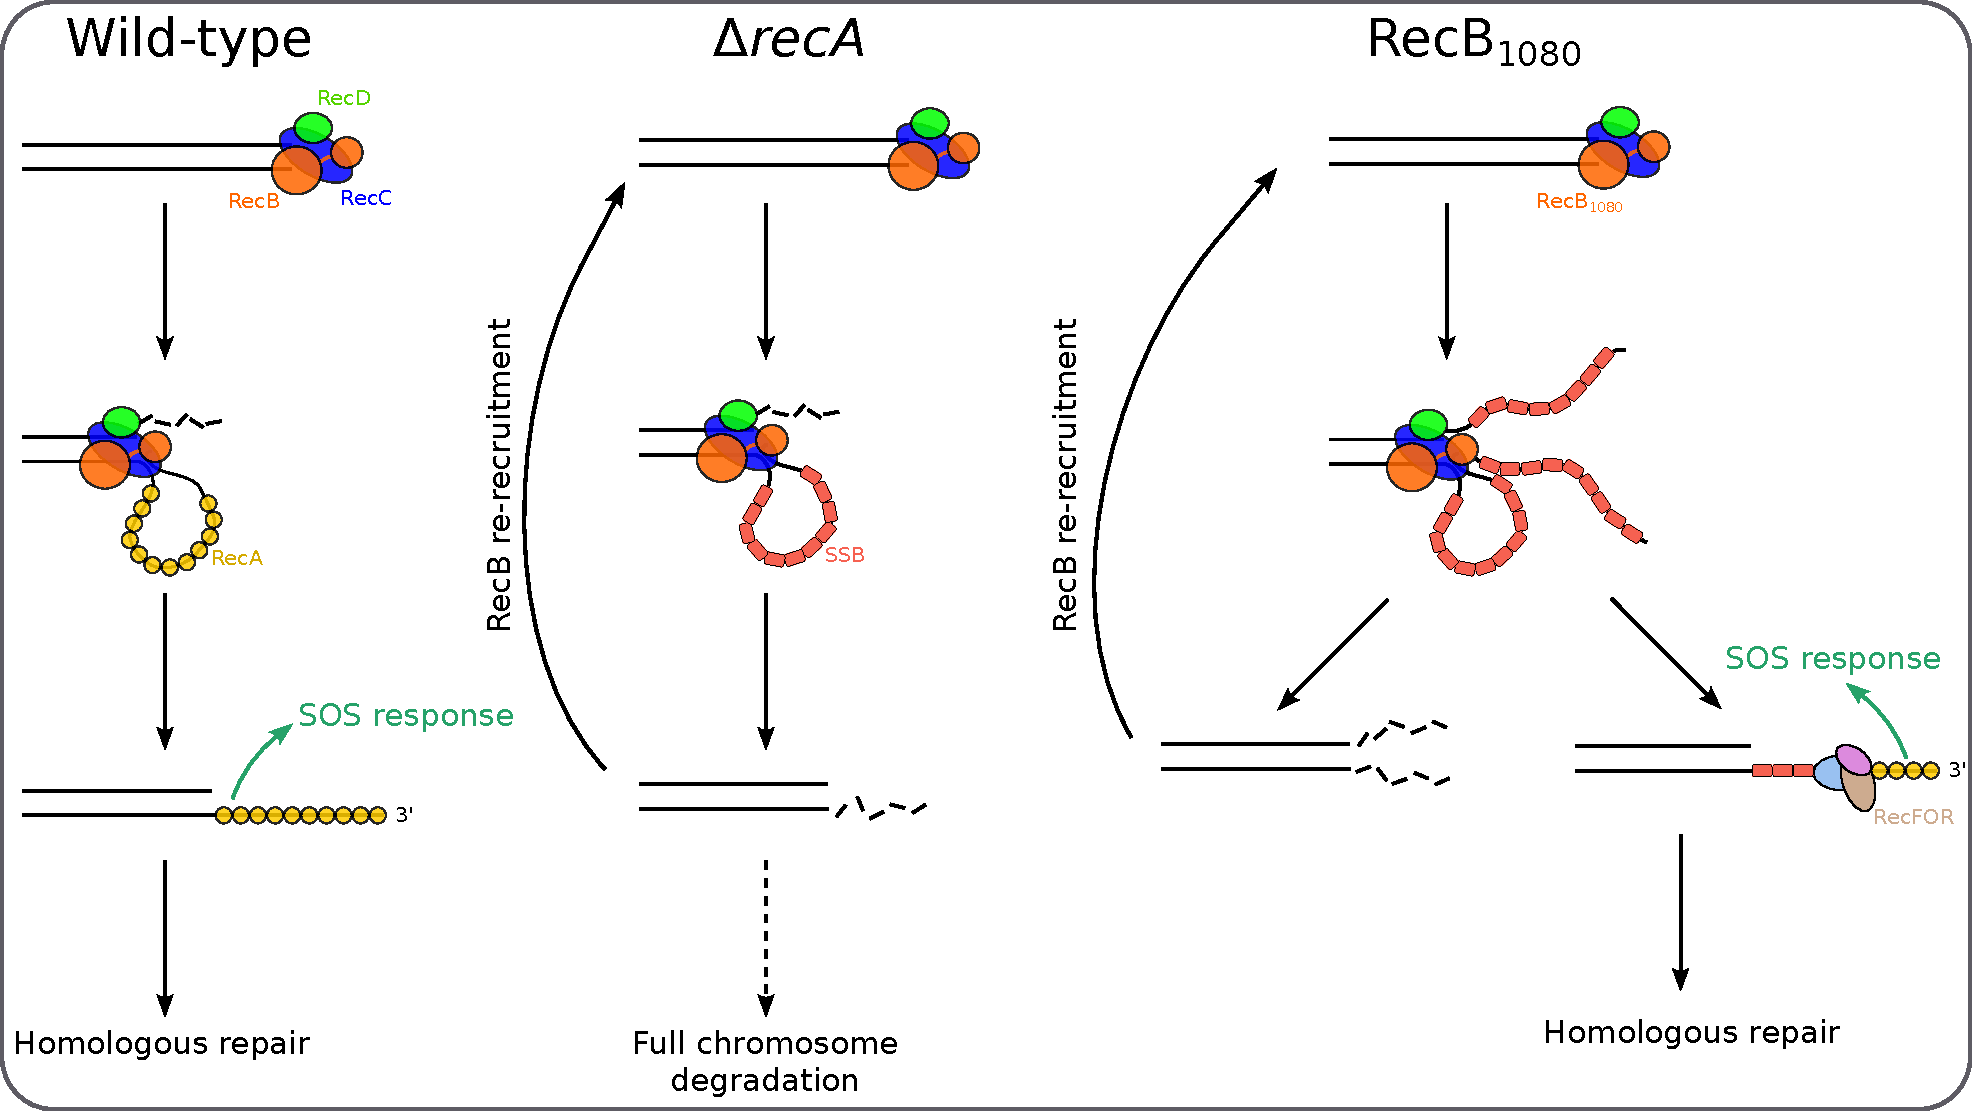
\includegraphics[width=\textwidth]{Figures/Fig_mutants_pathways.pdf}
    \caption{RecBCD recruitment pathways in wild-type \emph{E. coli}, \dreca\ and \geneteneighty\ mutants. \textbf{(Wild-type)} After DSB recognition, RecBCD degrades DNA until it recognises a Chi-site. It switches activity to create a 3' ssDNA overhang, and promotes RecA loading. The RecA-coated ssDNA can then be used for DNA repair by homologous recombination. \textbf{($\mathbf{\Delta}$reca)} In the absence of RecA, the 3' ssDNA is coated by SSB, and eventually digested by cellular nucleases. Blunting of the DNA end by digestion of the ssDNA creates a new substrate for binding of RecBCD. \textbf{(RecB$\mathbf{_{1080}}$)} Following DSB recognition, \teneighty\ unwinds DNA without digesting it. The unwound ssDNA can either be digested by nucleases, leading to a new blunt dsDNA end and RecBCD re-recruitment; or the RecFOR complex displaces SSB to load RecA, allowing DNA repair by homologous recombination to proceed.}
    \label{Fig:pathways}
\end{figure*}

Our observations of RecB recruitment to DSBs (Figure \ref{Fig:recruitment}) and nucleoid position (Figure \ref{Fig:nucleoid}) in the different mutant strains have led us to the model of RecB recruitment described in Figure \ref{Fig:pathways}, which confirms the model we previously proposed in \cite{Lepore2025}, and extends it by proposing that RecBCD gets reloaded multiple times on the same DSB. In wild-type cells, a DSB is recognised by RecBCD, which promotes RecA loading. The RecA filament triggers the SOS response, and is used for homology search and repair. In the \dreca\ mutant, the 3' ssDNA generated by RecBCD is first coated by SSB, and then degraded by the SbcCD and ExoI nucleases \cite{Zahradka2009}. This leads to blunting of the DNA end, creating a new substrate on which RecBCD can bind. This cycle likely leads to multiple RecBCD recruitments per DSB, and eventually to full chromosome degradation. In the \geneteneighty\ mutant, RecBCD unwinds DNA without degrading it. Our data show that at equal levels of DNA damage induction, \teneighty\ is recruited to the DSBs less frequently than RecBCD in \dreca\ cells (Figure \ref{Fig:recruitment}C, 8.5 $\pm$ 1.7 for \teneighty\ and 28.8 $\pm$ 9.5 for \dreca). This suggests that in the \geneteneighty\ mutant two competing pathways take place: either DNA degradation by SbcCD and ExoI leading to DNA-end blunting and re-recruitment of RecBCD; or RecA loading by RecFOR, leading to SOS induction and homologous repair. Thus the RecFOR-dependent pathway would provide an escape route from the cycle of re-recruitment.

\subsection*{RecA filaments accumulate under high DNA damage}
Under exposure to high ciprofloxacin concentrations (20-30 ng/ml), we observed an accumulation of cells that contained a RecA filament (Supp. Figures \ref{SIFig:reca_structures}A and \ref{SIFig:reca_structures}B). At these ciprofloxacin concentrations, we have determined that cells undergo frequent DSBs, leading to multiple recruitments of RecB to DSBs over the course of the experiment (up to 8 per hour, Figure \ref{Fig:recruitment}A). Given RecBCD's high processivity \cite{Wiktor2018}, such a high number of RecB recruitments would likely result in several tens of kilobases of DNA being digested at different chromosomal locations, which could result in the complete absence of a homologous copy of the DSB site. In this case, we expect that the repair process will stall at the homology search stage, after formation of the RecA filament, which is consistent with our observation that a large proportion of cells contain RecA filaments following exposure to high ciprofloxacin concentrations.

\subsection*{RecB colocalises with the bacterial nucleoid}
Imaging RecB simulteanously to the bacterial nucleoid reinforced our interpretation that long-lived RecB spots ($>$10 sec) are DSB-bound RecB molecules, and helped us understand their spatial distribution in the cell. As expected, DSB-bound RecB molecules moved to the centre of the cell after DSBs formation and colocalised with the nucleoid. Nucleoid compaction due to SOS induction and RecN activity had previously been reported after UV irradiation and mitomycin C \cite{Odsbu2014,Vickridge2017}, and we were able to confirm that a similar compaction occurs under ciprofloxacin treatment (Supp. Figure \ref{SIFig:nucleoid_compaction}). In the \dreca\ mutants, the lack of nucleoid compaction pointed out the involvement of RecA loading and SOS induction in nucleoid compaction, again confirming previous observations \cite{Odsbu2014,Vickridge2017}. In the \geneteneighty\ mutant, the nucleoid is more centred than in the wild-type strain but we did not observe any additional compaction upon exposure to ciprofloxacin. This could result from a substantial delay in SOS induction and recN expression as a result of the loading of RecA by the RecFOR alternative pathway \cite{Lepore2025}.

Taken together, this work provides a detailed picture of RecBCD's interaction with DNA following DSBs. We found that RecB dissociation is independent of RecA but depends on RecB's exonuclease activity, and that binding time is unaffected by DNA damage levels. Additionally, we observed changes in nucleoid conformation in response to DNA damage and examined the effects of high antibiotic levels on the formation of RecA filaments. The model we developed offers an overview of RecBCD recruitment to DSBs and dissociation from DNA, depending on the strain's ability to effectively carry out or complete repair.
These findings contribute valuable insights into the dynamics of DNA repair mechanisms in \ecoli, suggesting that RecBCD dissociation from DNA is an intrinsic property of the complex, largely unaffected by external factors, such as DNA damage levels or RecA loading.